\section{Domain Specific Languages}
A \ac{DSL} is a small programming language that focus on a particular domain \cite{fowler2010domain}. They stand in opposition to \acp{GPPL} (Java, C and so alike). \cite{beyak2011saga} define a set of advantages of using a \ac{DSL}:
\begin{itemize}
    \item Productive
    \item Comfortable
    \item Usable
    \item Integratable
    \item Low overhead
\end{itemize}
\cite{fowler2010domain} underline that \acp{DSL} have the advantage that they increase productivity and improve communication between domain experts and programmers. In a game development context, this would mean that designers and developers can communicate more easily \cite{Walter:2011:IDL:2071423.2071475}. Another benefit is that non-programmers can take part in the development \cite{beyak2011saga,Walter:2011:IDL:2071423.2071475}. 
\cite{Walter:2011:IDL:2071423.2071475} classify a good \ac{DSL} as a language that \dquote{features exactly the elements necessary to describe its domain}, meaning that it's easy to learn and may resemble spoken languages to some degree.

\subsection{External and internal DSLs}
\acp{DSL} are categorised into two categories; internal and external \cite{fowler2010domain}. An internal \ac{DSL} is an extension of a host language (e.g. Fluent \acp{API}, see \lstref{request:fluent}). External \acp{DSL} have their own distinct syntax and thus a separate language toolchain. External \acp{DSL} are integrated into the host language in the form of \acp{AST} or by generating code from the \ac{AST} in the host language \cite{fowler2010domain}.

\begin{lstlisting}[language={CSharp}, caption={Example of a Fluent \ac{API} to build a web request. Inspired by \cite{apache:fluent}}, label=lst:request:fluent]
FluentRequests.Post("http://host/")
        .WithTimeout(1000)
        .WithBody(...)
        .AddHeader("Authorization", ...)
        .OnOkResponse(resp => {
            //Process the response
        })
        .OnError(error => {
            //Handle the error
        }).
        .Send();
\end{lstlisting}

\subsection{DSLs in game development}
In order to understand the role of \acp{DSL} in game development, we have examined two \acp{DSL}; SCUMM and SAGA. SCUMM is a popular \ac{DSL} that was used through the eighties and nineties in several games \cite{fandon:scumm} and SAGA \cite{beyak2011saga} is an academic \ac{DSL} for story management. Afterwards we discuss the development method presented in \cite{Walter:2011:IDL:2071423.2071475}, that revolves around the use of \acp{DSL} in game development. Finally we created a tiny external \ac{DSL}, pca, to get a better understanding of how to implement a \ac{DSL} and a scene player for it.

\subsubsection{SCUMM}
SCUMM, which stands for Script Creation Utility for Maniac Mansion, is a \ac{DSL} created for Maniac Mansion by LucasArts \cite{gamasutra:scumm}. Maniac Mansion \cite{moby:mm} is a point-and-click adventure game where the player controls a character by clicking on things in the scene to trigger different events, such as unlocking new areas and picking up items. SCUMM was created to ease development. \acp{DSL} can improve productivity by enabling creative artists, such as the quest and story designers, to create their part of the game without assistance from a programmer \cite{gamasutra:scumm}. This is very beneficial because most game development teams have many creative artists, who do not have education/experience with programming, but are instead experts in designing quests or writing stories. 

\begin{lstlisting}[caption={An example of a SCUMM script},label=lst:scumm]
actor sandy face-right
actor sandy do-animation reach
walk-actor razor to-object microwave-oven
start-script watch-edna
stop-script
stop-script watch-edna
say-line dave "Don't be a tuna head."
say-line selected-kid "I don't want to use that right now."
\end{lstlisting}
\lstref{scumm} shows the syntax used in SCUMM, and how to start (line 4) and stop (line 5 and 6) other scripts from inside any script.

\subsubsection{SAGA}
The SAGA (Story as an Acyclic Graph Assembly) \ac{DSL} \cite{beyak2011saga} was developed at McMaster University in loose collaboration with an unnamed game development company. The goal of the \ac{DSL} is to provide story writers with a tool that allow them to formulate their stories so they can be integrated into the game code and managed in a better way than traditional methods. The game company would earlier track story progress by flipping bits in a bit vector, where each bit represented an event in the story. SAGA provides an easy to read \ac{DSL} that can generate story-management code \cite{beyak2011saga}.

\begin{lstlisting}[caption={SAGA Syntax}, label=lst:saga-syntax]
STORY Some Name
    INITIAL First State
    
    SECTION One {
        First State GOES Second State WHEN Condition
    }
    
    SECTION Two {
        Third State GOES Fourth State WHEN Other Condition
    }
    
    WHERE {
        Second State GOES Third State WHEN Alternate Condition
    }
\end{lstlisting}

The syntax of SAGA can be seen in \lstref{saga-syntax}. SAGA reserves a small number of keywords, which are capitalised. All of the reserved keywords have been used in the example. The state names can be any combination of letters, numbers, whitespace and special characters. The only limitation is that the characters; \squote{\{}, \squote{\}} and \squote{,} are reserved and if a reserved word is used as state name it cannot be fully capitalised. The compiled output of SAGA is a number of classes in either C, C\# or Java. The classes are the behaviour specified by the author of the script and a management class that can be used to progress the story as well as provide information about it.

\subsection{Game development with \acp{DSL}}
In \cite{Walter:2011:IDL:2071423.2071475} the authors present a development method that integrates \acp{DSL} into the game development process. They suggest that each studio should create one or more \acp{DSL} that is tailored to the games developed at the given studio. They underline that the \acp{DSL} should be sufficiently small to actually cover only a single domain (such as story telling, dialog building or similarly). 

The authors define two roles in the development process; the domain expert and the language engineer. The domain expert is responsible for defining entities and semantics in the language domain. The language engineer will integrate these into the language and design tools that ease the use of the language.

This process is carried out in an agile manner, meaning that the language will evolve as the requirements for the game changes. This method provides the game designers with a highly specialised and capable set of \acp{DSL} to aid them in the development.



\subsection{Visual Programming Languages}
Another type of \acp{DSL} are \acp{VPL}. A \ac{VPL} is a language defined with all the interaction as visual building blocks that can be linked together to create object or behaviour. \acp{VPL} makes it possible for game developers without textual programming experience.

One example of a \ac{VPL} is Unreal Engine's Blueprint system. In figure \ref{fig:unreal:blueprint} and example of these building blocks, and the linking of these building blocks, are shown.

\begin{figure}[H]
    \centering
    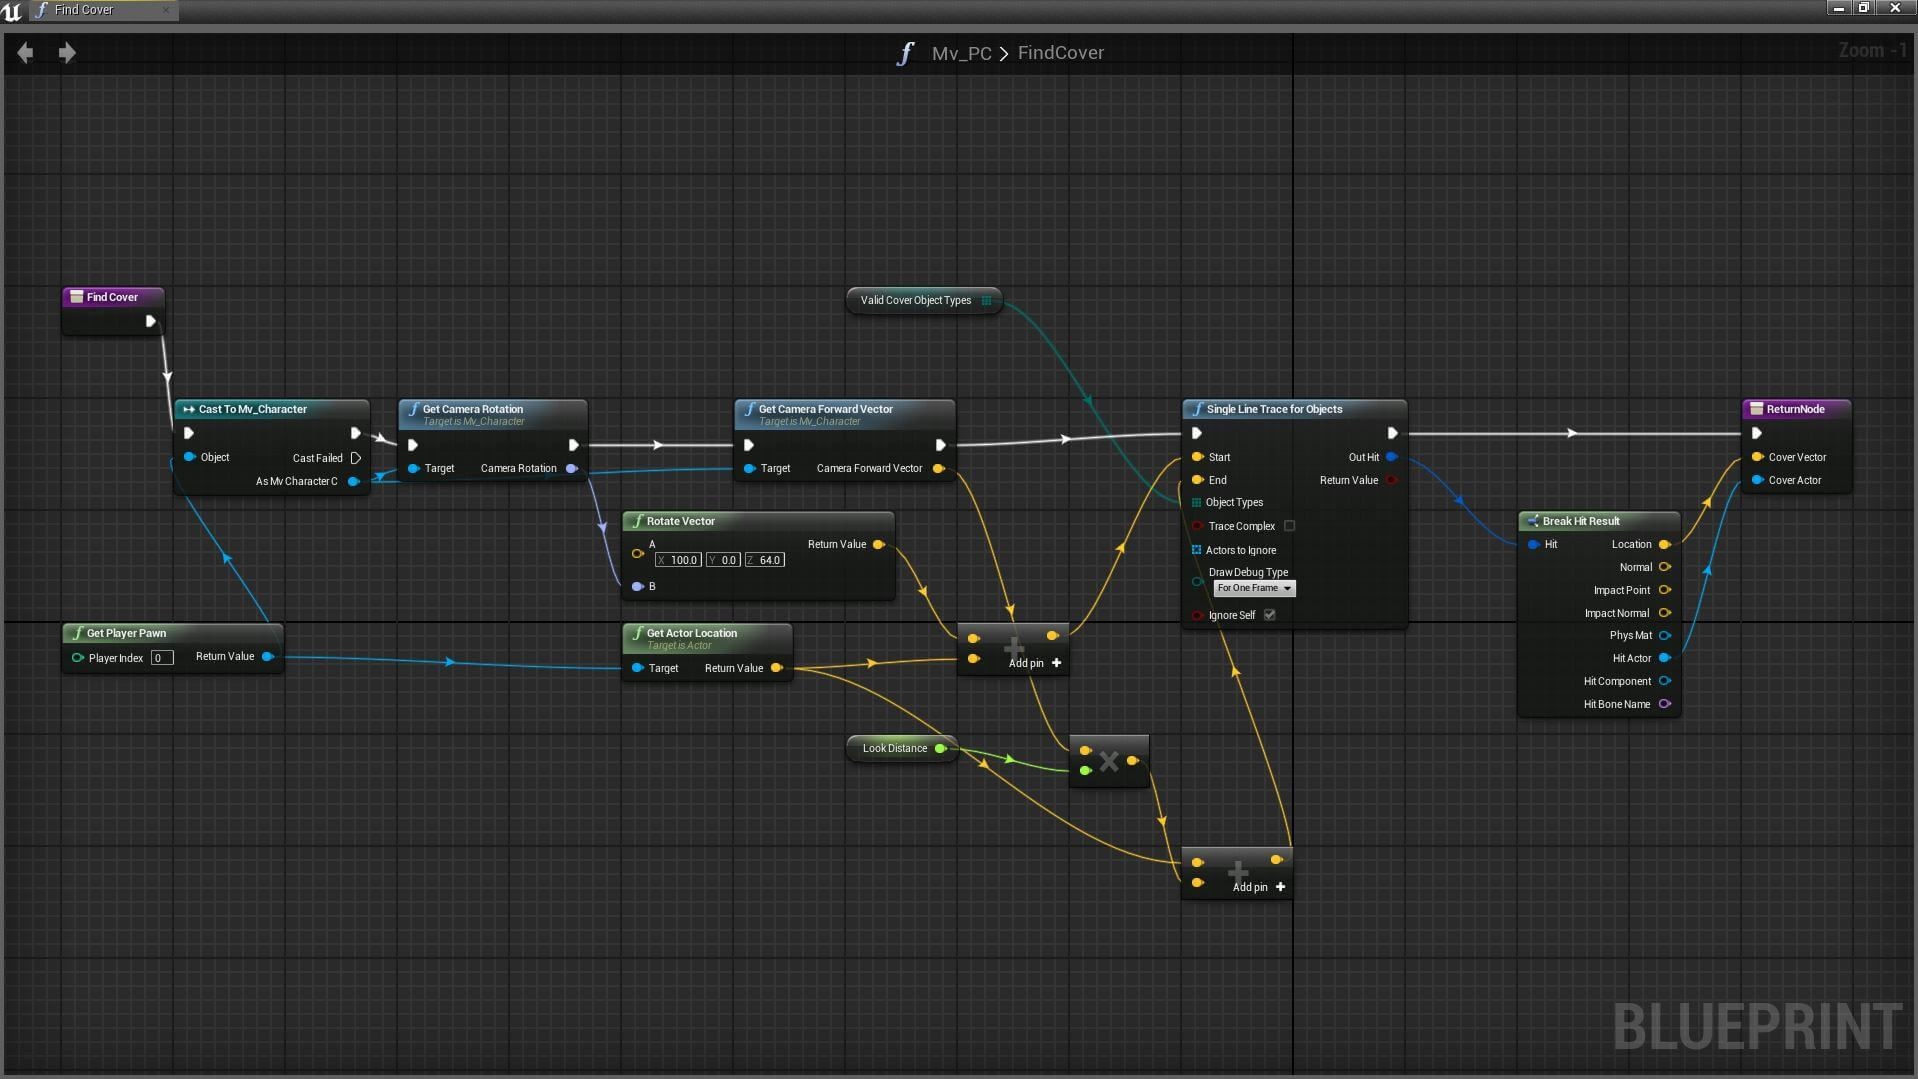
\includegraphics[width=\textwidth]{images/unreal_blueprint.jpg}
    \caption{An Example of Unreal Engine's Blueprint visual programming language}
    \label{fig:unreal:blueprint}
\end{figure}

Unreal Engine has this Blueprint system as a built-in, but similar tools exist for Unity though only third-party. For Unity there exists many competing solutions, with some of the 


\subsection{The DSL pca} \label{sec:animools}
In order to better understand \acp{DSL} we have developed an external \ac{DSL} called pca \cite{github:pca}, for creating point-and-click adventures, hence the name. It is external because it has a parser that generates an \ac{AST}. This \ac{AST} is imported by the host language, JavaScript, and executed.

pca may be used to place sprites on a background and have these be interactive through click events. The language is structured so that each source code file represents a scene.
Each scene consists of a background image and a number of sprite-models, each of which can be interactive through various actions on clicking on them. 

\subsection{Implementation of pca}
pca is implemented using a \ac{PEG} \cite{ford2004parsing}, and the parser was generated using the library PEG.js \cite{peg:js}. PEG.js requires the entire grammar for the lexer and parser to be specified in the same file using a custom syntax with embedded JavaScript. The grammar can be found in \appendixref{pca:grammar}. The parser outputs an \ac{AST}, which is loaded by the \dquote{engine} when it starts. The engine is a simple webpage with the background image specified in pca and some JavaScript implementing the placement of sprites and the various click handlers.

\lstref{pca:script} shows and example of a pca script. This script places a sprite of a house and a deer at specified positions in the scene. Each sprite has defined click handlers, so they are somewhat interactive. A click handler consists of one of several actions that are chained either sequentially or in parallel.

When the house is clicked, the reaction depends on whether the player has the key or not. If the player has the key, the scene will change to the scene located at \texttt{scenes/inside\_shed}.
When the \texttt{deer} is clicked and the player has completed \texttt{deerQuest1} it will say a couple of lines and then give the player a key to the shed. This means that the deer quest must be completed before progressing to the \texttt{inside\_shed}-scene.

The sprites' reactions to a click can be chained with two operators; \ttt{-\textgreater} and \ttt{\&}. The \ttt{-\textgreater} executes two actions sequentially and \ttt{\&} executes two actions in parallel. 

\begin{lstlisting}[caption={pca script to place a house and a deer sprite}, label={lst:pca:script}]
Scene 'in the meadows' with background 'backgrounds/fields_1.png' 
            with resolution 1280x720

Placeholder deerQuest1 = 'find apple for the deers'

Object 'house' with sprite 'sprites/shed.png' and size 0.6 at (750, 525)

Interaction with 'house' {
  if player has 'key to shed' {
    go to scene 'scenes/inside_shed'
  }
  else {
    display 'the door is locked, it might require a key to open'
  }
}

Actor 'big deer' with sprite 'sprites/deer.svg' and size 1.2 at (858, 570)

Interaction with 'big deer' {
  if objective deerQuest1 completed {
    'big deer' says 'thank you so much for the apple!' ->
    'big deer' says 'you can have this key' ->
    'big deer' says 'i found it near that tree over there' &
    player receives 'key to shed' ->
    'big deer' moves to (-80, 568) over 8s
  }
  else {
    'big deer' gets 'hungry' &
    'big deer' says "i'm hungry" &
    'big deer' moves to (805, 568) over 1s ->
    'big deer' moves to (878, 568) over 1.5s ->
    'big deer' moves to (872, 568) over 0.3s
  }
}
\end{lstlisting}

